\chapter{\IfLanguageName{dutch}{Stand van zaken}{Quantum Essentials}}
\label{ch:quantum-essentials}

To make sure everyone starts off on the same baseline to understand the full potential of this paper, we will introduce a few of the basic quantum principles. This paper is not targeting these specific principles but they are essential to be able to learn more about quantum computing and its potential. If there is any specific interest regarding these ground fundamentals, we would like to refer you to the following papers, ~\textcite{Rieffel1998} and ~\textcite{Shor2000}.

\section{The Qubit and its representations}

The foundation of any quantum related paper is and always will be the \textbf{qubit}. A qubit is just like a classical computing \textbf{bit}: the foundational unit of the quantum computer. Whilst a bit can either be on or off, a qubit has a certain statistical measurement to it. This statistical aspect is derived from the way we interact with a measurement of a qubit. Now keeping this in mind, to be able to program on a quantum computer you need to be able to encode classical problems in a quantum manner, which as it turns out is not an easy task.

A qubit is not an infinite on or off, meaning that any type of computation needs to happen during the time frame that the qubit remains stable without being thrown of its state by decoherence (2.0.3) or any other external factors. In other words defining a qubit as being on or off is simply not enough, if we want to keep the time-factor in the equation.
One of the biggest issues with qubits is that they can behave unstable when influenced by the slightest of external factors, which also means the influence of an external observer. Once a qubit reaches an unstable state it has lost its quantum advantages and becomes a determined particle, making it unavailable for calculations. Meaning that during the execution of your program you are simply not able to look at the intermediary results as this would affect the final result, which would make the whole computation unreliable.

Now more defined, to comprehend the nature of a qubit we need to understand that representing a qubit is only possible in a complex field, which visualises a certain amplitude of the state of the qubit at a certain point in time. When thinking about a classical bit, we like to imagine a switch being turned on or off. With a qubit you would have to think about a sphere that is being transformed and shifted around its axes to transform its state. \textit{Felix Bloch} was the individual that came up with the Bloch sphere that we currently use to clearly represent what state a qubit is in at a certain point in time. Looking at figure 2.1 you are able to see a representation of the state of a qubit in its elevated state. You need to think about this representation in a complex field on which transformations and rotations can be applied.
During runtime a qubit is in a probabilistic state where it can not be fully determined in which state the qubit currently resides, which makes the whole execution harder. The moment we measure the state of the qubit it will degrade back to a determined result that shows us exactly the state of the qubit, but in turn loses the quantum potential initially gained.

\begin{figure}[h]
	\centering
	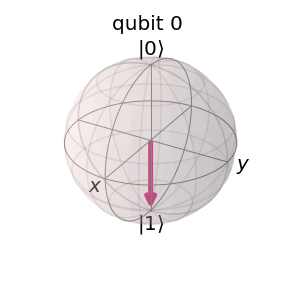
\includegraphics[scale = 0.75]{../Demonstration/img/Quantum_essentials_1.PNG}
	\caption{A Bloch sphere representation of a qubit in the elevated $\ket{1}$ state. 
		The Bloch sphere clearly indicates that the state of a qubit has a complex aspect to it. By representing it in a sphere, we are able to showcase how the direction of the arrow also defines its probabilistic state. In this case the arrow has a probability of 1.00 for the elevated $\ket{1}$ state.}
\end{figure}

Another way of demystifying what a qubit exactly means is by representing it through the use of matrices and the Bra-ket notation. By using these matrices and using matrix transformations we can more easily expose the way a qubit can be influenced during execution. 
If you take a look at the way of representing a qubit in its elevated $\ket{1}$ state or ground $\ket{0}$ state in the formulae below, we are able to look at qubits in a more mathematical manner. Also by representing the qubits as a matrix we are able to more clearly show how operations on a quantum device have an impact on the state of the qubit.


\[
	\ket{0}=
	\begin{bmatrix}
	1					\\
	0
	\end{bmatrix} 
	and
	\ket{1}=
	\begin{bmatrix}
	0					\\
	1
	\end{bmatrix} 
\]

These formulae are mostly preferred by computer scientists because it gives them a clear image of the transformations, much in the same way an ordinary logic gate can influence an electrical signal. The combination of qubit basis states can be achieved by the utilisation of a Kronecker product. In the formulae below you are able to see how a 2-qubit system is represented through their matrix-representation. So look at the following transformations in much the same way one would look at an electrical signal that flows through a set of classical gates.

\[
\ket{00}=
\begin{bmatrix}
1					\\
0
\end{bmatrix} 
\otimes
\begin{bmatrix}
1					\\
0
\end{bmatrix} =
\begin{bmatrix}
1					\\
0					\\
0					\\
0					\\
\end{bmatrix}
\quad
\ket{01}=
\begin{bmatrix}
1					\\
0
\end{bmatrix} 
\otimes
\begin{bmatrix}
0					\\
1
\end{bmatrix} =
\begin{bmatrix}
0					\\
1					\\
0					\\
0					\\
\end{bmatrix}
\]
\[
\ket{10}=
\begin{bmatrix}
0					\\
1
\end{bmatrix} 
\otimes
\begin{bmatrix}
1					\\
0
\end{bmatrix} =
\begin{bmatrix}
0					\\
0					\\
1					\\
0					\\
\end{bmatrix}
\quad
\ket{11}=
\begin{bmatrix}
0					\\
1
\end{bmatrix} 
\otimes
\begin{bmatrix}
0					\\
1
\end{bmatrix} =
\begin{bmatrix}
0					\\
0					\\
0					\\
1					\\
\end{bmatrix}
\]

To sum it up a bit can be only be in a state of on or off and this can be checked throughout execution, whilst a qubit is in a uncertain state during execution much like Schrödinger's cat. So once we observe the qubit it becomes just as determined as a normal bit would be. But determining the state during execution will affect the rest of the experiment and will remove the potential benefits of quantum in much the same way if Schrödinger continued the experiment after observation that the cat had died. he would then have the certainty that the cat would still be dead at a later point in time.

\section{Superposition and entanglement}

Now the next 2 principles are fully responsible for giving quantum computing its exponential speed-up potential compared to classical computing in certain tasks like factorisation and database searches. However these principles only offer that powerful advantage when they operate together in solving a certain quantum algorithm. 

\subsection{Superposition}
\textbf{Superposition} is a widely used term that gets thrown around a lot without any proper explanation, so what it exactly represents is the real question.

We should think about qubits in superposition in a statistical manner to receive a clearer image of what the term superposition means before performing any calculations. When a qubit is put into a state of superposition, the qubit operates between its elevated state $\ket{1}$ and its ground state $\ket{0}$. Referring back to the representation of the Bloch sphere the qubit lives in a three dimensional complex field, where the only knowledge we can keep track of, is its statistical chance of the state of the qubit at a certain point in time. Until we have truly observed the qubit and have measured it extensively, the state of a qubit remains a statistical probability.

This all meaning that a quantum particle in superposition can remain in both states at once statistically whilst it has yet not been observed. To explain this more clearly from a computer science perspective, a qubit in superposition is during execution behaving as 0 and 1 at the same time. A concept that seems impossible within a classical frame of mind but a concept that can also be very advantageous. E.g. if you are processing a big array of data through your classical processor, your processor will take one item of the array, process, convert and output it before it will take another item of the array and perform the same thing. A quantum processor could go about this process in a similar yet much more ingenious way. It would put an amount of qubits in superposition to represent the full array as input, perform the needed amount of quantum gates and receive the output in a single go instead of needing to loop over the full array. ~\autocite{Draper2000} Using a graphical processing unit does allow classical devices to perform in a likewise parallel manner, but it still does not do this through 1 computational cycle because you still need to combine the results at the end of the process.

\subsection{Entanglement}
\textbf{Entanglement} is another interesting principle within the realm of quantum physics. This principle truly offers the quantum advantage that is predicted over every single sector. 
It refers to the correlation between entangled qubits where the state of one qubit influences the state of the correlated qubit in a way that it can be exploited and theoretically exponentially speed up computation. This entanglement can be achieved inside a quantum computer by the use of quantum gates on qubits in a state of superposition. You are able to put every single qubit available in a entangled state with the qubits available in the system. 

E.g. when we have a 3-qubit system, we are able to entangle every single qubit with each other and put them in a superposition state as to be able to play around with the quantum capabilities of our system. Now let us add a single qubit to this system. By adding this single qubit we are able to entangle this qubit with the 3 other qubits. So this addition of the qubit has added the qubit itself as a new possible data-point into the system but it has also added these 3 new states of entanglement which in itself are new data-points. 

This phenomenon is the reason why a quantum computer has an exponential factor to any added qubits, it becomes more clear where the quantum advantage can truly be gained. Such a quantum system can represent an immense amount of classical bits by using this phenomenon. The deterministic result of the computation with the qubits at the end of an experiment will always reflect the correlations of the qubits in the results. Furthermore we must keep in mind that enough experiments are to be performed in order to defend against the possible mistakes of external influences on a quantum system.
~\autocite{fern2016mathematics}

\subsection{Quantum advantage}
Superposition and entanglement are constantly being used by a quantum processor to achieve a quantum advantage as the one that Google showed of in their latest showcase of their 'quantum supremacy', ~\textcite{Google2019}. they are able to exponentially increase the computing power of a quantum computer, as you add more qubits you are exponentially increasing the available data items that kind of processor could handle. 

E.g. to be able to simulate the most known medicine of the 20th century, penicillin, one would need 286 functional qubits, which in turn would be able to generate the $2^{286}$ bits of memory. It is impossible to gather enough classical RAM in the whole world to be able to simulate this drug exactly ($1.30 * 10^{50}$ atoms on earth approximately). If we were able to simulate any type of drug exactly, but as of now quantum computers are not capable of holding this amount of stable and reliable qubits. So actually getting to such a stable amount of qubits in itself would need a new breakthrough in the way we can add stable qubits to a system. The whole limitation of 'just adding qubits' to the system runs into a barrier by a term called Quantum decoherence.

\section{Quantum decoherence}

QC is not solely composed of benefits, the biggest downside is that as of now technology has not yet progressed far enough to actually provide the necessary amount of stable qubits to perform trustworthy calculations. For example for the simulation of penicillin, a system would need 286 qubits that remain stable for a prolonged period. But as of now  Google has only been able to keep 53 qubits stable for a prolonged period of time using quantum error correction throughout the calculations. The loss of these quantum aspects during execution is called \textit{quantum decoherence}, it is the phenomenon that describes how a qubit falls in an unstable state after being influenced by external forces or even internal influences from the qubits around it inside the system.

Referring to figures 2.2 and 2.3 we are able to see that decoherence is a measurable phenomenon. The circuit below is especially built to show that decoherence shows up in the smallest of computations. In figure 2.2 a qubit gets thrown in an elevated state of $\ket{1}$ and then gets measured and pictured on a classical bit. Looking at the results you are able to see that quantum decoherence has occurred and de-elevated the state of the qubit back to $\ket{0}$ in 8\% of the cases. In this experiment, were we have taken 1024 shots performing the circuit on the real quantum device, around 8 percent or 81 of the shots, were influenced to its ground state due to the quantum decoherence. For the code used for the generation of this figure, we refer to appendix A. 

Taking all of this into account the whole field has one giant, non-circumventable downside. The larger our quantum systems become, the more internal decoherence we receive from the higher concentration of qubits near each other. This all could mean that there is a limit to how big we are able to make quantum machines. Because at a certain point, without proper error correction, the internal decoherence would make every single calculation useless because of the high probability of faulty data throughout. However if we are able to find a solution to this internal decoherence, the amount of qubits inside a system could be limitless and our data processing with it could also become limitless. \autocite{Hartnett2019}

It is of utmost importance that we add qubits in a controlled manner where we are able to perform better error-correction before we add more qubits into the system. If qubits would start to be added to the systems without performing any research regarding quantum error correction, we would only receive an increase in quantity of computing power not in its reliability. And in this case quality is a more important factor compared to quantity.

\begin{figure}[h]
	\centering
	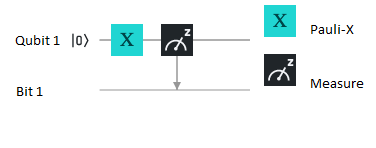
\includegraphics[scale = 0.75]{../Demonstration/img/Quantum_decoherence_circuit.PNG}
	\caption{This is the quantum circuit that puts a qubit in an elevated state using the Pauli-X gate followed up with a measurement, to show off how quantum decoherence influences the results.}
\end{figure}

\begin{figure}[h]
	\centering
	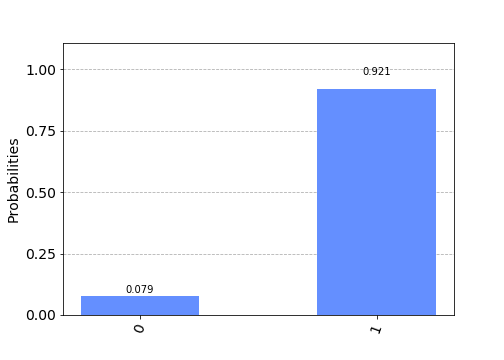
\includegraphics[scale = 0.75]{../Demonstration/img/Quantum_decoherence_graph.PNG}
	\caption{These are the percentages after performing the circuit on a real device from which it is visible that quantum decoherence has taken place on the initial $\ket{1}$ state to the $\ket{0}$ state.}
\end{figure}



\section{Quantum gates}

How do we create calculations with particles that are not observable and not tangible at a specific point in time. Quantum gates offer the solution to this question, a quantum gate affects one or more qubits during execution so that a programmer is able to perform changes to the state of the qubit but does not necessarily create an unstable qubit. From a programmers perspective they function in a similar way that a normal logic gate functions on an electrical signal inside a regular processor. 

A major rule that a quantum computer needs to adhere  to when it comes to its gates, is that quantum computations have to be 100 percent reversible in comparison to a classical computer that does not have to deal with this limitation. This is clearly shown when we use the matrix representations of a qubit that passes through a specific quantum gate. Because by the very nature of quantum mechanics operations on these matrices are unitary and by that also reversible.

E.g. think of an OR-gate where you are able to only see the outcome of the signal with an on or an off signal. Now you can not know just from the outcome alone which initial signal influenced the OR-gate to be activated. This shows that a classical device is not bound by this gate-reversibility limitation. Now you can look at these gates in two different perspectives. First in the three dimensional perspective, we could apply a rotation over the z-axis of +90 to the qubit, now by the very nature of a rotation we could apply the reverse of this previous operation and receive the same state of the qubit initially. Secondly we have the option of representing these qubits by the Bra-ket notation and its accompanied matrix notation. A quantum gate would apply its unitary transformation mathematically to the state of a qubit. And by the very definition of an Unitary transformation, they are reversible. Both of these perspectives are viable to explain quantum aspects.

To understand the application of quantum gates during runtime on a quantum computer, we would like to refer solely back to the representation of matrices where unitary transformations are applied by performing a Kronecker product on the qubit in question.

\subsection{Hadamard gate}
The Hadamard gate is the single most important gate for creating a quantum computation. This gate is responsible for putting a qubit inside a state of superposition and is also is the one to get it out of this state. So in turn without this gate, quantum advantage would simply not exist. It maps  $\ket{0}$ to $\frac{\ket{0} + \ket{1}}{\sqrt{2}}$ and $\ket{1}$ to $\frac{\ket{0}-\ket{1}}{\sqrt{2}}$, which are both superposition states.

\[
H=\frac{1}{\sqrt{2}}\begin{bmatrix}
1 & 1 \\
1 & -1
\end{bmatrix}
\]

\subsection{Pauli-X gate}
Performs in a similar way a classical NOT-gate performs on an electrical signal or an absence of it. A qubit in $\ket{0}$ state going through a Paul-X gate would go in a $\ket{1}$ state. We also showcase an example on how we apply these unitary transformations when the qubit would pass through a gate of this type.

\[
X=
\begin{bmatrix}
0 & 1 \\
1 & 0
\end{bmatrix}
\]

\[
PauliX * \ket{0}=
\begin{bmatrix}
0 & 1 \\
1 & 0
\end{bmatrix}
*
\begin{bmatrix}
1 \\
0
\end{bmatrix}
=
\begin{bmatrix}
0 \\
1
\end{bmatrix}
=
\ket{1}
\]

\[
PauliX * \ket{1}=
\begin{bmatrix}
0 & 1 \\
1 & 0
\end{bmatrix}
*
\begin{bmatrix}
0 \\
1
\end{bmatrix}
=
\begin{bmatrix}
1 \\
0
\end{bmatrix}
=
\ket{0}
\]
\subsection{CNOT gate}
This gate works as a flip for a qubit. It is a gate that connects two qubits together, where one is the control qubit and the other the target. If the control qubit is in an activated state it will flip the target qubit.

 \[
 CNOT=
 \begin{bmatrix}
 1 & 0 & 0 & 0 \\
 0 & 1 & 0 & 0 \\
 0 & 0 & 0 & 1 \\
 0 & 0 & 1 & 0 \\	
 \end{bmatrix}
 \]

\subsection{Toffoli, CCNOT gate}
The Toffoli gate works in the same way as a CNOT gate, but instead it has 2 control qubits. So both of them need to be activated to actually flip the target qubit, which logically requires at least 3 qubits in your system. This gate is the connector of the whole quantum system where we are able to entangle states in superposition.

 \[
CCNOT=
\begin{bmatrix}
1 & 0 & 0 & 0 & 0 & 0 & 0 & 0\\
0 & 1 & 0 & 0 & 0 & 0 & 0 & 0\\
0 & 0 & 1 & 0 & 0 & 0 & 0 &  0\\
0 & 0 & 0 & 1 & 0 & 0 & 0  & 0\\
0 & 0 & 0 & 0 & 1 & 0 & 0  & 0\\
0 & 0 & 0 & 0 & 0 & 1 & 0  & 0\\
0 & 0 & 0 & 0 & 0 & 0 & 0 & 1 \\
0 & 0 & 0 & 0 & 0 & 0 & 1 & 0\\
\end{bmatrix}
\]

This is just a listing of the most prevalent quantum gates. These quantum gates form the basis for performing the simplest of quantum algorithms. These can be implemented through a programming interface or through many of the UI-editors where you can add gates along the circuit in a dynamic way. You are even able to send off these generated circuits through the UI tools to any real devices or simulators to analyse and compare your results.



